
%(BEGIN_QUESTION)
% Copyright 2005, Tony R. Kuphaldt, released under the Creative Commons Attribution License (v 1.0)
% This means you may do almost anything with this work of mine, so long as you give me proper credit

Beregn alle spenningsfall og strømmer i denne kretsen, med piler for strømretning og polaritetsmerking for spenningspolariteter. Beregn deretter total spenningsforsterkning i denne forsterkerkretsen ($A_V$), både som forholdstall og som verdi i desibel (dB):

$$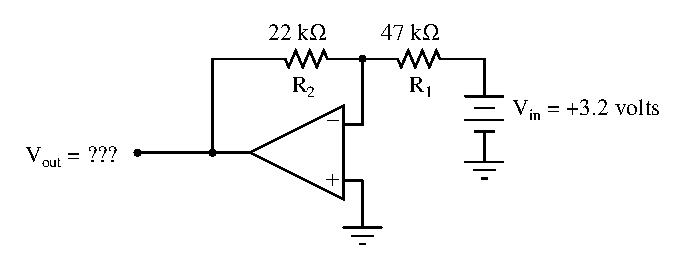
\includegraphics[width=15.5cm]{i01475x01.eps}$$

\vskip 20pt \vbox{\hrule \hbox{\strut \vrule{} {\bf Forslag til sokratisk diskusjon} \vrule} \hrule}

\begin{itemize}
\item{} Identifiser ``forenklende antakelser'' vi vanligvis bruker når vi analyserer DC-opampkretser. Tips: én handler om virkningen av negativ tilbakekobling på inngangsspenningene, og en annen handler om strøm i inngangsterminalene.
\item{} Forklar hvordan denne kretsen vil oppføre seg hvis 22 k$\Omega$-motstanden feiler åpen.
\item{} Forklar hvordan denne kretsen vil oppføre seg hvis 22 k$\Omega$-motstanden feiler kortsluttet.
\item{} Forklar hvordan denne kretsen vil oppføre seg hvis 47 k$\Omega$-motstanden feiler åpen.
\item{} Forklar hvordan denne kretsen vil oppføre seg hvis 47 k$\Omega$-motstanden feiler kortsluttet.
\item{} Forklar hvordan denne kretsen vil oppføre seg hvis op-ampens (+)- og ($-$)-innganger byttes om.
\end{itemize}

\underbar{file i01475}
%(END_QUESTION)





%(BEGIN_ANSWER)

$$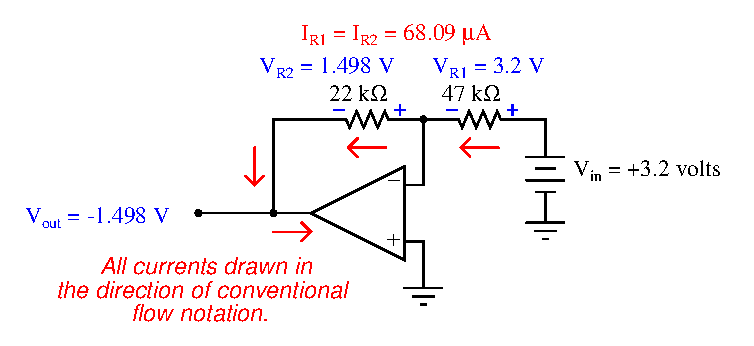
\includegraphics[width=15.5cm]{i01475x02.eps}$$

$A_V$ = 0.468 = -6.594 dB

%(END_ANSWER)





%(BEGIN_NOTES)

Operasjonsforsterkerkretser gir en god mulighet til å repetere grunnleggende begreper i likestrømskretser: spenningsfall, polaritet, strømretning, Ohms lov, Kirchhoffs spenningslov, Kirchhoffs strømlov osv. Denne kretsen er intet unntak. Vektlegg at svært mange op-amp-kretser kan analyseres fullstendig kun med disse grunnprinsippene og egenskapene til en ideell op-amp (null inngangsstrøm, uendelig åpen sløyfeforsterkning, ubegrenset utgangssving og null spenning mellom inngangsterminalene når negativ tilbakekobling er virksom).

Noen studenter kan komme fram til feil forsterkningsverdi fordi de blindt følger en formel med $R_1$ og $R_2$ som variabler, og setter inn kretsens verdier uten å vurdere hvilken motstand som er hvilken (er $R_1$ tilbakekoblingsmotstanden, eller er det $R_2$?). Dette er med hensikt, fordi jeg vil at studentene skal lære å {\it tenke} over hva de gjør i stedet for å følge instrukser tankeløst.




\vfil \eject

\noindent
{\bf Oppsummeringsquiz:}

Beregn strømmen gjennom motstanden $R_1$ i denne op-amp-kretsen:

$$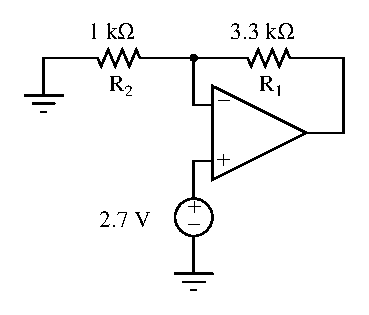
\includegraphics[width=15.5cm]{i01475x03.eps}$$

\begin{itemize}
\item{} 0.812 mA
\vskip 5pt 
\item{} 0.628 mA
\vskip 5pt 
\item{} 11.6 mA
\vskip 5pt 
\item{} 6.21 mA
\vskip 5pt 
\item{} 2.70 mA
\vskip 5pt 
\item{} 8.91 mA
\end{itemize}


%INDEX% Electronics review: opamp inverting amplifier circuit

%(END_NOTES)

